%%%%%%%%%%%%%%%%%%%%%%%%%%%%%%%%%%%%%%%%%%%%%%%%%%%%%%%%%%%%%%%%%%
%%%%%%%% ICML 2017 EXAMPLE LATEX SUBMISSION FILE %%%%%%%%%%%%%%%%%
%%%%%%%%%%%%%%%%%%%%%%%%%%%%%%%%%%%%%%%%%%%%%%%%%%%%%%%%%%%%%%%%%%

% Use the following line _only_ if you're still using LaTeX 2.09.
%\documentstyle[cs541,epsf,natbib]{article}
% If you rely on Latex2e packages, like most moden people use this:
\documentclass{article}

% use Times
\usepackage{times}
% For figures
\usepackage{graphicx} % more modern
%\usepackage{epsfig} % less modern
\usepackage{subcaption}
\usepackage{amsmath}

% For citations
\usepackage{natbib}

% For algorithms
\usepackage{algorithm}
\usepackage{algorithmic}

% As of 2011, we use the hyperref package to produce hyperlinks in the
% resulting PDF.  If this breaks your system, please commend out the
% following usepackage line and replace \usepackage{cs541} with
% \usepackage[nohyperref]{cs541} above.
\usepackage{hyperref}

% Packages hyperref and algorithmic misbehave sometimes.  We can fix
% this with the following command.
\newcommand{\theHalgorithm}{\arabic{algorithm}}

\usepackage[accepted]{cs541}


% The \icmltitle you define below is probably too long as a header.
% Therefore, a short form for the running title is supplied here:
\icmltitlerunning{Enhanced Residual Context-based Networks for Image Outpainting}

\begin{document} 

\twocolumn[
\icmltitle{Enhanced Residual Context-based Networks for Image Outpainting}

% It is OKAY to include author information, even for blind
% submissions: the style file will automatically remove it for you
% unless you've provided the [accepted] option to the icml2017
% package.

% list of affiliations. the first argument should be a (short)
% identifier you will use later to specify author affiliations
% Academic affiliations should list Department, University, City, Region, Country
% Industry affiliations should list Company, City, Region, Country

% you can specify symbols, otherwise they are numbered in order
% ideally, you should not use this facility. affiliations will be numbered
% in order of appearance and this is the preferred way.
\icmlsetsymbol{equal}{*}

\begin{icmlauthorlist}
\icmlauthor{Przemek Gardias}{wpi}
\icmlauthor{Eric Arthur}{wpi}
\icmlauthor{Huaming Sun}{wpi}
\end{icmlauthorlist}

\icmlaffiliation{wpi}{Worcester Polytechnic Institute}

\icmlcorrespondingauthor{}{\{pmgardias, etarthur, hsun2\}@wpi.edu}

% You may provide any keywords that you 
% find helpful for describing your paper; these are used to populate 
% the "keywords" metadata in the PDF but will not be shown in the document
\icmlkeywords{image outpainting, generative adversarial network, context encoder, computer vision, deep learning, machine learning, ICML}

\vskip 0.3in
]

% this must go after the closing bracket ] following \twocolumn[ ...

% This command actually creates the footnote in the first column
% listing the affiliations and the copyright notice.
% The command takes one argument, which is text to display at the start of the footnote.
% The \icmlEqualContribution command is standard text for equal contribution.
% Remove it (just {}) if you do not need this facility.

\printAffiliationsAndNotice{}  % leave blank if no need to mention equal contribution
%\printAffiliationsAndNotice{\icmlEqualContribution} % otherwise use the standard text.
%\footnotetext{hi}

\begin{abstract} 
Although humans perform well at predicting what exists beyond the boundaries of an image, deep models struggle to understand context and extrapolation through retained information. This task is known as image outpainting and involves generating realistic expansions of an image’s boundaries. Current models use generative adversarial networks to generate results which lack localized image feature consistency and appear fake. We propose two methods to improve this issue: the use of a local and global discriminator, and the addition of residual blocks within the encoding section of the network. Comparisons of our model and the baseline’s L1 loss, MSE loss, and qualitative differences reveal our model is able to naturally extend object boundaries and produce more internally consistent images compared to current methods but produces lower fidelity images.
\end{abstract} 

\section{Introduction}
The use of generative adversarial models has led to many new developments in the computer vision field. The task known as image inpainting, which aims to enhance or restore quality to parts of an image, requires a model to retain the context of the image while completing missing regions of the image, and iteratively improve the process of the generations. The problem explored in this paper is a significantly more ambiguous task than its inpainting alternative, and is commonly known as image outpainting. For this task, the input image boundaries are extrapolated outside of the original content of the input based upon the context of the image.\cite{sabini_painting_2018}

\begin{figure}
	\captionsetup[subfigure]{labelformat=empty}
    \centering
    \begin{subfigure}[b]{0.15\textwidth}
        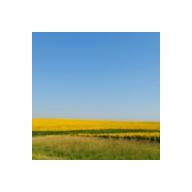
\includegraphics[width=\textwidth]{figs/fig1/masked_input}
        \caption{Masked input}
    \end{subfigure}
    \hfill
    \begin{subfigure}[b]{0.15\textwidth}
        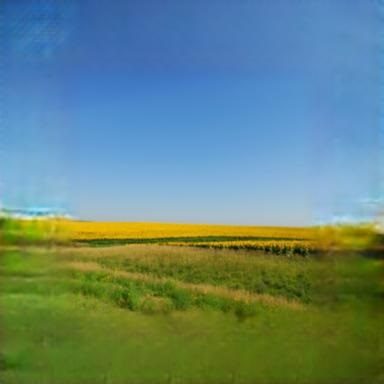
\includegraphics[width=\textwidth]{figs/fig1/baseline}
        \caption{Output}
    \end{subfigure}
    \hfill
    \begin{subfigure}[b]{0.15\textwidth}
        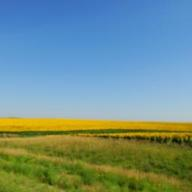
\includegraphics[width=\textwidth]{figs/fig1/ground_truth}
        \caption{GT}
    \end{subfigure}
  	\caption{Example of image outpainting.}
  	\label{fig:fig1}
\end{figure}

Image outpainting, sometimes referred to as image context interpretation and extrapolation, requires the context of the image to be retained by the encoder to accurately re-generate the known input image, then create new portions to append to the edges of the image as shown in Figure \ref{fig:fig1}. There exists research on this task using GANs, however one of the biggest issues with image outpainting is the new additions to the image, known as hallucinations, typically appear lower quality than the base image and therefore can easily be distinguished as fake by the human eye.\cite{sabini_painting_2018} Therefore, to effectively create higher quality hallucinations, better image evaluation methods are required to match the discrimination abilities of human interpretation.

\subsection{Research contributions}
We provide insight into the use of a local discriminator alongside a global discriminator to improve the quality of hallucinations, additionally evaluating the performance of residual blocks applied to the context encoder portion of our generative network. 

\section{Related Work}
In this section, we briefly review the previous works relating to this paper in three sub-fields: Generative Adversarial Networks, Image Inpainting, and Image Outpainting.

\subsection{Generative Adversarial Networks}
Deep generative models have shown success in various tasks of image and video generation problems. By training the generator and discriminator in tandem, the generator can capture the real data distribution and create more realistic images given the latent input. However, GANs are often prone to collapse and are difficult to train. Therefore, some newer techniques have been applied attempting to reduce this issue such as the addition of residual blocks to the encoder component of the generator specifically researched within a super-resolution task context.\cite{lim_enhanced_2017}

\subsection{Image Inpainting}
Image inpainting is the task of recovering missing regions or enhancing regions within images. Pathak et al. demonstrate that context encoder can achieve realistic results for generation of novel images sections for inpainting purposes.\cite{pathak_context_2016} Recent improvements include applying global and local discriminators to improve the generated feature consistency within the missing sections of the input image by identifying poor generations only within the area of the inpainted sections.\cite{iizuka_globally_2017} Liu et al. more recently apply partial convolutions to improve overall consistency of generated images.\cite{liu_image_2018}

\section{Proposed Method}
In this section, we provide an overview of our architecture. Since the task is generative we use a GAN which other current methods employ. Our GAN is based on the architecture provided by Van Hoorick with two major additions: the first being the use of residual blocks in the generator, and the second being the use of two discriminators.\citep{van_hoorick_image_2020} Below we explore the exact architecture and some design decisions behind it.

\subsection{Generator}
We propose a GAN architecture that aims to encode the context of the image and use deconvolutional layers to then generate the resulting image while retaining feature consistency. We apply a residual model to the generative network, first convolving the image down into its feature space, then using deconvolution to upsample the image into its expanded version. Although typical models that contain residual blocks often include batch normalization within the blocks, we do not include this activation layer per demonstrations of improvement in the deblurring work of Nah et al.\cite{nah_deep_2018} The encoder section of the generative network contains multiple residual blocks in an attempt to improve image quality. Table \ref{tab:1} outlines the layers of our generative network, including both the encoder and decoder components.

\begin{table}[h] 
  \centering  
    \begin{tabular}{lcc}  
    \hline
    \textbf{layer} & \textbf{output size} & \textbf{parameters}\\ 
    \hline \hline
      Conv & 16$\times$192$\times$192 & 5$\times$5, stride=1 \\
    \hline
      ResBlock & 128$\times$96$\times$96 & 3$\times$3, stride=2 \\
    \hline
      ResBlock & 256$\times$48$\times$48 & 3$\times$3, stride=2 \\
    \hline
      ResBlock & 256$\times$48$\times$48 & 3$\times$3, stride=1 \\
    \hline
      ResBlock & 256$\times$48$\times$48 & 3$\times$3, stride=1 \\
    \hline
      ResBlock & 256$\times$48$\times$48 & 3$\times$3, stride=1 \\
    \hline
      Conv & 256$\times$48$\times$48 & 3$\times$3, stride=1 \\
    \hline
      ReLU & 256$\times$48$\times$48 & None \\
    \hline
      Conv & 256$\times$48$\times$48 & 3$\times$3, stride=1 \\
    \hline
      ReLU & 256$\times$48$\times$48 & None \\
    \hline
      Conv & 256$\times$48$\times$48 & 3$\times$3, stride=1 \\
    \hline
      ReLU & 256$\times$48$\times$48 & None \\
    \hline
      Trans-Conv & 128$\times$96$\times$96 & 4$\times$4, stride=1 \\
    \hline
      ReLU & 128$\times$96$\times$96 & None \\
    \hline
      Conv & 128$\times$96$\times$96 & 3$\times$3, stride=1 \\
    \hline
      ReLU & 128$\times$96$\times$96 & None \\
    \hline
      Trans-Conv & 64$\times$192$\times$192 & None \\
    \hline
      ReLU & 64$\times$192$\times$192 & None \\
    \hline
      Conv & 32$\times$192$\times$192 & 3$\times$3, stride=1 \\
    \hline
      ReLU & 32$\times$192$\times$192 & None \\
    \hline
      Conv & 3$\times$192$\times$192 & 3$\times$3, stride=2 \\
    \hline
      Sigmoid & 3$\times$192$\times$192 & None \\
    \hline
    \end{tabular}
  
  \caption{Architecture of generator $G$, including parameters. Trans-Conv is transposed convolution.} 
  \label{tab:1} 
\end{table}

\begin{table}[h] 
  \centering  
    \begin{tabular}{lc}  
    \hline
    \textbf{Layer} & \textbf{Parameters}\\ 
    \hline \hline
      Conv & 3$\times$3, stride=$s_{in}$ \\
    \hline
      ReLU & None \\
    \hline
      Conv & 3$\times$3, stride=$s_{in}$ \\
    \hline
      ReLU & None \\
    \hline
      Add & None \\
    \hline
    \end{tabular}
  
  \caption{Architecture of residual block used in generator $G$, including parameters. The residual block applies input strides $s_{in}$ to the convolution layer. Add is an element-wise addition of block input tensor $x$ and output tensor of previous layer.} 
  \label{tab:2}
\end{table}

\subsection{Discriminator}
Our discriminator network $D$ consists of dual discriminators. One discriminator $D_G$ takes as input the entire generated image and applies a convolutional network to identify the image as real or generated, while the second discriminator $D_L$ is local, and is restricted solely to the boundaries between the input image and the hallucinations. These discriminator outputs are averaged, meaning our total discriminator network output is 

\begin{align}
	D(x) &= \frac{D_L(\mu \times x) + D_G(x)}{2}
\end{align}

where $\mu$ is the binary mask which is originally applied to the training images.

The purpose of the local discriminator is to attempt to remove the clearly fake hallucinations that result from pixel noise or manifestations, that to the human eye are clearly fake. Since these happen in the boundary between the input image and the hallucinations, the local discriminator focuses on these areas alone as shown in Table \ref{tab:3}.

\begin{table}[h] 
  \centering  
    \begin{tabular}{lc}  
    \hline
    \textbf{Layer} & \textbf{Parameters}\\ 
    \hline \hline
      Conv & 3$\times$3, stride=2 \\
    \hline
      InstanceNorm & None \\
    \hline
      LeakyReLU & negative slope=0.2 \\
    \hline
      Conv & 3$\times$3, stride=2 \\
    \hline
      InstanceNorm & None \\
    \hline
      LeakyReLU & negative slope=0.2 \\
    \hline
      Conv & 3$\times$3, stride=2 \\
    \hline
      InstanceNorm & None \\
    \hline
      LeakyReLU & negative slope=0.2 \\
    \hline
      Conv & 3$\times$3, stride=2 \\
    \hline
      InstanceNorm & None \\
    \hline
      LeakyReLU & negative slope=0.2 \\
    \hline
      Conv & 3$\times$3, stride=1 \\
    \hline
      InstanceNorm & None \\
    \hline
      LeakyReLU & negative slope=0.2 \\
    \hline
      Conv & 3$\times$3, stride=1 \\
    \hline
    \end{tabular}
  
  \caption{Architecture of global and local discriminators $D_G$ and $D_L$, respectively.} 
  \label{tab:3}
\end{table}

\section{Experiment}
Describe the computational experiments you conducted to validate the approach you took.

Training is done for 50 epochs, with a fixed learning rate of $\alpha=0.0003$ and two Adam optimizers with $\beta_1=0.5, \beta_2=0.999$, following the same hyperparameters proposed in Van Hoorick 2020 \cite{van_hoorick_image_2020} The loss functions are as follows:

\begin{align}
  L_{rec} &= ||x-G(x)||_1 \\
  L_{adv} &= ||D(G(x))-1||_2^2 \\
  L_G &= \lambda_{rec}L_{rec} + \lambda_{adv}L_{adv} \\
  L_D &= ||D(x)-1||_2^2 + ||D(G(x))-0||_2^2
\end{align}

We apply a time based remedy to the generator loss function that punishes the generator heavier for bad outputs as time progresses.

\begin{align}
  \lambda_{adv}(n) = \begin{cases}
    0.001, & \text{if }n\leq10 \\
    0.005, & \text{if }10<n\leq30 \\
    0.015, & \text{otherwise}
  \end{cases}
\end{align}

Since humans still perform vastly greater than deep learning networks at this task we conclude our experiment with a qualitative discussion about the quality of hallucinations. As many previously mentioned models in this domain create noise or lines that are clearly out of place in the hallucinations, we aim to manually evaluate whether our model rectifies this issue or these manifestations are still present.

\section{Results}
Describe the results of the experiments, including their immediate implications (e.g., ``the result suggests that technique A performs better than technique B''). If your work is purely theoretical, then this section (as well as the previous section) might be replaced with mathematical proofs.

\begin{table}[h] 
  \centering  
    \begin{tabular}{lrrr}
    \hline
    \textbf{Model} & \textbf{L1} & \textbf{MSE} & \textbf{Adversarial}\\ 
    \hline \hline
      Baseline & $0.0956$ & $0.047$ & $0.1278$ \\
      Local Discriminator & $0.897$ & $1.044$ & $0.1014$ \\
      Residual Encoder & $0.08$ & $0.7814$ & $0.0941$ \\
    \hline
    \end{tabular}
  
  \caption{TODO} 
  \label{tab:4}
\end{table}

\begin{figure*}
	\captionsetup[subfigure]{labelformat=empty}
    \centering
    \begin{subfigure}[b]{0.175\textwidth}
        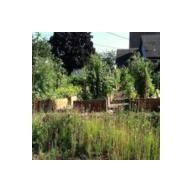
\includegraphics[width=\textwidth]{figs/fig2/masked_input}
        \caption{Masked input}
    \end{subfigure}
    \hfill
    \begin{subfigure}[b]{0.175\textwidth}
        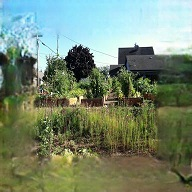
\includegraphics[width=\textwidth]{figs/fig2/baseline}
        \caption{Baseline}
    \end{subfigure}
    \hfill
    \begin{subfigure}[b]{0.175\textwidth}
        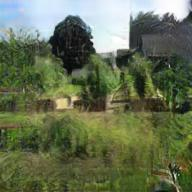
\includegraphics[width=\textwidth]{figs/fig2/local}
        \caption{Discriminator}
    \end{subfigure}
    \hfill
    \begin{subfigure}[b]{0.175\textwidth}
        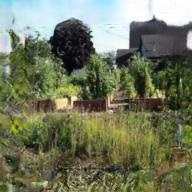
\includegraphics[width=\textwidth]{figs/fig2/residual}
        \caption{Residual}
    \end{subfigure}
    \hfill
    \begin{subfigure}[b]{0.175\textwidth}
        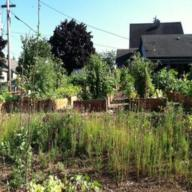
\includegraphics[width=\textwidth]{figs/fig2/ground_truth}
        \caption{GT}
    \end{subfigure}
  	\caption{Comparison of results for different model variants.}
  	\label{fig:fig2}
\end{figure*}

\begin{figure}
	\captionsetup[subfigure]{labelformat=empty}
    \centering
    \begin{subfigure}[b]{\textwidth}
        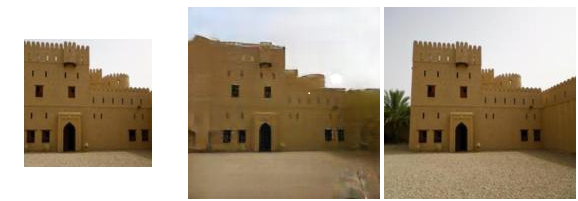
\includegraphics[width=\textwidth]{figs/fig3/fig3}
        \caption{
        	\begin{tabular}{ccc}
        	Masked input & Local & GT
        	\end{tabular}
        }
    \end{subfigure}
  	\caption{Outpainting example using local discriminator model.}
  	\label{fig:fig3}
\end{figure}

\begin{figure}
	\captionsetup[subfigure]{labelformat=empty}
    \centering
    \begin{subfigure}[b]{\textwidth}
        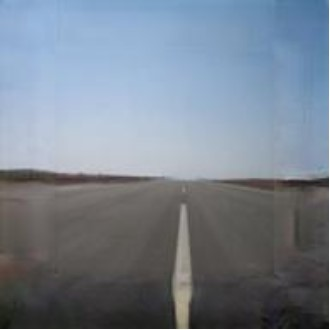
\includegraphics[width=\textwidth]{figs/fig4/fig4}
    \end{subfigure}
  	\caption{Outpainting result example using residual encoder model.}
  	\label{fig:fig4}
\end{figure}

\begin{figure}
	\captionsetup[subfigure]{labelformat=empty}
    \centering
    \begin{subfigure}[b]{\textwidth}
        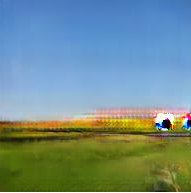
\includegraphics[width=\textwidth]{figs/fig5/fig5}
    \end{subfigure}
  	\caption{Example of anomaly with the hallucination.}
  	\label{fig:fig5}
\end{figure}

\section{Discussion}
Describe limitations of your work as well as further-ranging implications (e.g., ``our work suggests that doing XYZ in general may be a useful approach to...'').

\section{Conclusions and Future Work}
Briefly summarize the key findings your paper and point out interesting directions for future inquiry.

\bibliography{paper.bib}
\bibliographystyle{cs541}

\end{document} 


% This document was modified from the file originally made available by
% Pat Langley and Andrea Danyluk for ICML-2K. This version was
% created by Lise Getoor and Tobias Scheffer, it was slightly modified  
% from the 2010 version by Thorsten Joachims & Johannes Fuernkranz, 
% slightly modified from the 2009 version by Kiri Wagstaff and 
% Sam Roweis's 2008 version, which is slightly modified from 
% Prasad Tadepalli's 2007 version which is a lightly 
% changed version of the previous year's version by Andrew Moore, 
% which was in turn edited from those of Kristian Kersting and 
% Codrina Lauth. Alex Smola contributed to the algorithmic style files.  
